\begin{frameO}[We want]

    A \emph{lot} of IoT devices want to access to a gateway (base station).

    \begin{itemize}\tightlist
        \item
              Insert them in a \textbf{crowded wireless network}.
        \item
              With a protocol \textbf{slotted in time and frequency}.
        \item
              Each device has a \textbf{low duty cycle} (a few messages per day).
    \end{itemize}

    \pause

    \only<1>{
        % \begin{figure}[!h]
            \centering
            \includegraphics[width=0.65\linewidth]{system_model1.eps}
            % \caption{In our system model, some dynamic devices (in the \textcolor{blue}{IoT network in blue}) transmit packets to a gateway and suffer from the interference generated by neighboring networks (in \textcolor{orange}{orange left/right}).}
            % \label{fig:41:system_model1}
        % \end{figure}
    }

    \only<2>{
        % \pause

        \begin{colorblock}{Goal}
            \begin{itemize}\tightlist
                \item Maintain a \textbf{good Quality of Service}.
                \item \textbf{Without} centralized supervision!
            \end{itemize}
        \end{colorblock}

        % \pause

        \begin{alertblock}{How?}
            \begin{itemize}\tightlist
                \item Use \textbf{learning algorithms}: devices will learn on which frequency they should talk!
            \end{itemize}
        \end{alertblock}
    }

\end{frameO}



\section{\hfill{}2. Model and hypotheses\hfill{}}

\subsection{\hfill{}2.a. Model\hfill{}}

\begin{frameO}[Model]

    \begin{itemize}\tightlist
        \item
              Discrete time \(t\geq1\) and \(K\) radio channels (\emph{e.g.}, 10)
              \hfill{} (\emph{known})
    \end{itemize}

    \begin{figure}[h!]
        \centering
        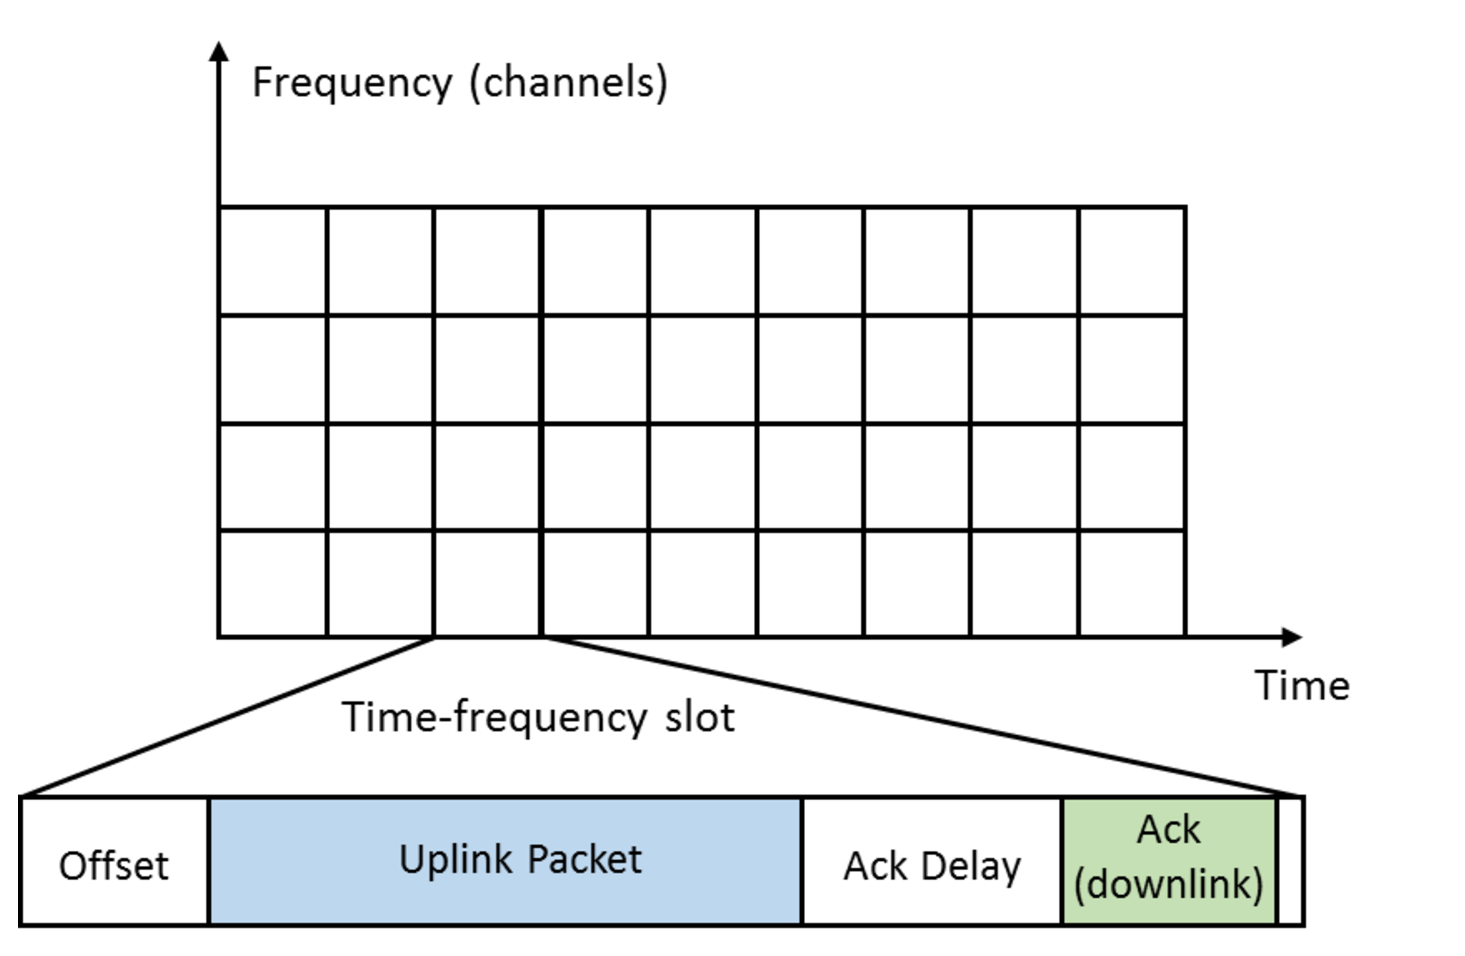
\includegraphics[height=0.35\textheight]{protocol.eps}\\
        {\small Chosen protocol : \textcolor{blue}{uplink messages $\nearrow$} followed by \textcolor{darkgreen}{\emph{acknowledgements} $\swarrow$}.}
    \end{figure}

    \begin{itemize}\tightlist
        \item
              \(D\) \textbf{dynamic} devices try to access the network
              \emph{independently}
        \item
              \(S=S_1+\dots+S_{K}\) \textbf{static} devices occupy the network :
              \newline
              \(S_1,\dots,S_{K}\) in each channel \hfill{} (\emph{unknown}).
    \end{itemize}

\end{frameO}



\subsection{\hfill{}2.b. Hypotheses\hfill{}}

\begin{frameO}[Hypotheses ($1/2$)]

    \begin{colorblock}{Emission model}

        \begin{itemize}\tightlist
            \item
                  Each device has the same \emph{low} emission probability: \newline
                  each step, each device sends a packet with probability \(p\).
                  \newline
                  \hfill{}\small{(this gives a duty cycle proportional to $1/p$)}
        \end{itemize}

    \end{colorblock}

    \vspace*{20pt}

    \begin{lightblock}{Background traffic}

        \begin{itemize}\tightlist
            \item
                  Each static device uses only one channel.
            \item
                  Their repartition is fixed in time.
        \end{itemize}

        \(\implies\) This ambiant traffic bothers the dynamic devices!
    \end{lightblock}

\end{frameO}

\begin{frameO}[Hypotheses ($2/2$)]

    \begin{colorblock}{Dynamic radio reconfiguration}

        \begin{itemize}\tightlist
            \item
                  Each \textbf{dynamic device decides the channel to use to send every
                      packet}.
            \item
                  It has memory and computational capacity to implement a basic decision
                  algorithm.
        \end{itemize}

    \end{colorblock}

    \vspace*{20pt}

    \begin{lightblock}{Problem}

        \begin{itemize}\tightlist
            \item
                  \emph{Goal} : \emph{maximize packet loss ratio} (\(=\) number of
                  received \texttt{Ack}) in a \emph{finite-space discrete-time Decision
                      Making Problem}.
            \item
                  \emph{Solution ?} \textbf{Multi-Armed Bandit algorithms},
                  \textbf{decentralized} and used \textbf{independently} by each device.
        \end{itemize}

    \end{lightblock}

\end{frameO}



\section{\hfill{}3. Baseline algorithms\hfill{}}

\subsection{\hfill{}3.a. A naive strategy : uniformly random access\hfill{}}

\begin{frameO}[A naive strategy : uniformly random access]

    \begin{itemize}\tightlist
        \item
              \textbf{Uniformly random access}: dynamic devices choose uniformly
              their channel in the pull of \(K\) channels.
        \item
              Natural strategy, dead simple to implement.
    \end{itemize}

    % \pause

    \begin{itemize}\tightlist
        \item
              Simple analysis, in term of \textbf{successful transmission
                  probability} (for every message from dynamic devices) :
    \end{itemize}

    \begin{small} \begin{align*}
            \mathbb{P}(\text{success}|\text{sent}) = \sum_{i=1}^{K} \underbrace{(1 - p / K)^{D-1}}_{\text{No other dynamic device}} \times \underbrace{(1-p)^{S_i}}_{\text{No static device}} \times\; \frac{1}{K}.
        \end{align*} \end{small}

    % \pause

    \begin{itemize}\tightlist
        \item
              Works fine only if all channels are similarly occupied,\newline
              but \textbf{it cannot learn} to exploit the best (more free)
              channels.
    \end{itemize}

\end{frameO}



\subsection{\hfill{}3.b. Optimal centralized strategy\hfill{}}

\begin{frameO}[Optimal centralized strategy]

    \begin{itemize}\tightlist
        \item
              If an oracle can decide to affect \(D_i\) dynamic devices to channel
              \(i\), the \textbf{successful transmission probability} is:
              \vspace*{-10pt}

              \begin{small} \begin{align*}
                      \mathbb{P}(\text{success}|\text{sent}) = \sum_{i=1}^{K} \underbrace{(1 - p)^{D_i - 1}}_{\;\;D_i - 1 \;\text{others}\;\;} \times \underbrace{(1 - p)^{S_i}}_{\;\;\text{No static device}\;\;} \times \underbrace{ D_i / D }_{\;\;\text{Sent in channel}\; i}.
                  \end{align*} \end{small}
        \item
              The oracle has to solve this \textbf{optimization problem}:
              \vspace*{-5pt}

              \begin{small} \begin{equation*} \begin{cases}
                          \underset{D_1,\dots,D_{K}}{\arg\max}\;\;\; & \sum_{i=1}^{K} D_i (1 - p)^{S_i + D_i -1}                                             \\
                          \text{such that}\;\;\;                       & \sum_{i=1}^{K} D_i = D \; \text{and} \; D_i \geq 0, \; \; \forall 1 \leq i \leq K .
                      \end{cases} \end{equation*} \end{small}
        \item
              We solved this quasi-convex optimization problem with \emph{Lagrange
                  multipliers}, only numerically.
        \item
              \(\implies\) Very good performance, maximizing the transmission rate
              of all the \(D\) dynamic devices.
    \end{itemize}

\end{frameO}

\begin{frameO}[Optimal centralized strategy]

    \begin{colorblock}{But unrealistic}

        But \textbf{not achievable in practice}:
        \begin{itemize}
            \item
            there is no oracle
            \item
            and there is no centralized supervision!
        \end{itemize}

    \end{colorblock}

    \begin{colorblock}{Let see \emph{realistic decentralized approaches}}

        \(\hookrightarrow\) Machine Learning ? \newline
        \hspace*{15pt}\(\hookrightarrow\) Reinforcement Learning ? \newline
        \hspace*{30pt} \(\hookrightarrow\) \emph{Multi-Armed Bandit} !

    \end{colorblock}

\end{frameO}



\section{\hfill{}4. Multi-Armed Bandit algorithm : UCB\hfill{}}

\subsection{\hfill{}4.1. Multi-Armed Bandit formulation\hfill{}}

\begin{frameO}[Multi-Armed Bandit formulation]

    A dynamic device tries to collect \emph{rewards} when transmitting :

    \begin{itemize}
        \tightlist
        \item
              it transmits following a Bernoulli process \newline
              (probability \(p\) of transmitting at each time step \(\tau\)),
        \item
              chooses a channel \(A(\tau) \in \{1,\dots,K\}\),
        \item
              if \texttt{Ack} (no collision) \hspace*{10pt} \(\implies\) reward
              \(r_{A(\tau)} = 1\),
        \item
              if collision (no \texttt{Ack}) \hspace*{10pt} \(\implies\) reward
              \(r_{A(\tau)} = 0\).
    \end{itemize}

    % \pause

    \begin{colorblock}{Reinforcement Learning interpretation}

        Maximize transmission rate \(\equiv\) \textbf{maximize cumulated
            rewards}
        \[\max_{\text{algorithm}\;A} \;\; \sum_{\tau=1}^{\text{horizon}} r_{A(\tau)}.\]

    \end{colorblock}

\end{frameO}

\subsection{\hfill{}4.2. Upper Confidence Bound algorithm : UCB\hfill{}}

\begin{frameO}[Upper Confidence Bound algorithm (\(\mathrm{UCB}_1\))]

    A dynamic device keeps \(\tau\) number of sent packets, \(T_k(t)\)
    selections of channel \(k\), \(X_k(t)\) successful transmission in
    channel \(k\).

    \begin{enumerate}
        \def\labelenumi{\arabic{enumi}.}
        \tightlist
        \item
              For the first \(K\) steps (\(\tau=1,\dots,K\)), try each channel
              \emph{once}.
        \item
              Then for the next steps \(t \geq K\) :

              \begin{itemize}
                  \tightlist
                  \item
                        Compute the index
                        \(\mathrm{UCB}_k(\tau) := \underbrace{\frac{X_k(\tau)}{N_k(\tau)}}_{\text{Mean}\; \widehat{\mu_k}(\tau)} + \underbrace{\sqrt{\frac{\log(\tau)}{2 N_k(\tau)}},}_{\text{Upper Confidence Bound}}\)
                  \item
                        Choose channel
                        \(A(\tau) = \mathop{\arg\max}\limits_{k} \; \mathrm{UCB}_k(\tau)\),
                  \item
                        Update \(T_k(\tau+1)\) and \(X_k(\tau+1)\).
              \end{itemize}
    \end{enumerate}

    \begin{colorblock}{Random activation?}
        \begin{itemize}
            \item
            The times $\tau$ are \textbf{not} the global time indexes $t$
            \item
            each object transmits only with probability $p$ at each time $t$
            \item
            (following its Bernoulli activation pattern)
        \end{itemize}
    \end{colorblock}

    % \vfill{}\hfill{}\tiny{\textcolor{gray}{References: [Lai \& Robbins, 1985], [Auer et al, 2002], [Bubeck \& Cesa-Bianchi, 2012]}}

\end{frameO}



\section{\hfill{}5. Experimental results\hfill{}}

\subsection{\hfill{}5.1. Experiment setting\hfill{}}

\begin{frameO}[Experimental setting]

    \begin{colorblock}{Simulation parameters}

        \begin{itemize}
            \tightlist
            \item
                  \(K = 10\) channels,
            \item
                  \(S + D = 10000\) devices in total,
            \item
                  \(p = 10^{-3}\) probability of emission,
            \item
                horizon \(T = 10^5\) total time slots (avg. \(\simeq 100\) messages \(/\)
                  device),
            \item
                  The proportion of dynamic devices \(D/(S+D)\) varies,
            \item
                  Various settings for \((S_1,\dots,S_{K})\) static devices
                  repartition.
        \end{itemize}

    \end{colorblock}

    \pause

    \begin{colorblock}{What do we show}

        \begin{itemize}
            \tightlist
            \item
                  After a short learning time, MAB algorithms are almost as efficient as
                  the oracle solution.
            \item
                  Never worse than the naive solution.
            \item
                  Thompson sampling is even more efficient than UCB.
        \end{itemize}

    \end{colorblock}

\end{frameO}



\subsection{\hfill{}5.2. First result: $10\%$\hfill{}}

\begin{frameO}[\(10\%\) of dynamic devices]

    \begin{figure}[h!]
        \centering
        \includegraphics[height=0.74\textheight]{10intelligent.eps}
        \caption{\small{$10\%$ of dynamic devices. Gives $7\%$ of gain.} {\tiny \textcolor{gray}{[Bonnefoi, Besson et al, CROWNCOM 2017], Ch.4.3}}}
    \end{figure}

\end{frameO}



\subsection{\hfill{}5.2. First result: $30\%$\hfill{}}

\begin{frameO}[\(30\%\) of dynamic devices]

    \begin{figure}[h!]
        \centering
        \includegraphics[height=0.74\textheight]{30intelligent.eps}
        \caption{\small{$30\%$ of dynamic devices. Gives $3\%$ of gain but not much is possible.}}
    \end{figure}

\end{frameO}



\subsection{\hfill{}5.3. Growing proportion of devices dynamic devices\hfill{}}

\begin{frameO}[Dependency on \(D/(S+D)\)]

    \begin{figure}[h!]
        \centering
        \includegraphics[height=0.65\textheight]{perf_learning.eps}
        \caption{\small{\emph{Almost optimal}, for any proportion of dynamic devices, \emph{after a short learning time}. Up-to $16\%$ gain over the naive approach!}}
    \end{figure}

\end{frameO}
